\documentclass{beamer}
\usepackage{etex}
\usetheme{Frankfurt}
\usepackage{amsmath}
\usepackage{amssymb}
\usepackage{bm}
\usepackage{extramarks}
\usepackage{amsfonts}
\usepackage{amsthm}
\usepackage{array}
\usepackage{xy}
\usepackage{multicol}
\usepackage{hyperref}
\usepackage{float}
\usepackage[algoruled]{algorithm2e}
\usepackage{subfig}
\usepackage{graphicx}
\setlength\parindent{0pt}
\usepackage{resizegather}
\addtobeamertemplate{navigation symbols}{}{%
    \usebeamerfont{footline}%
    \usebeamercolor[fg]{footline}%
    \hspace{1em}%
    \insertframenumber/\inserttotalframenumber
}

%%Set symbols
\newcommand{\given}{\ensuremath{|} }
\newcommand{\AND}{\ensuremath{\cap} }
\newcommand{\OR}{\ensuremath{\cup} }

\newcommand{\N}{\mathbb{N}}
\newcommand{\R}{\mathbb{R}}
\newcommand{\Z}{\mathbb{Z}}
\newcommand{\Q}{\mathbb{Q}}

\newcommand{\powerset}[1]{\ensuremath{ \mathcal P \left({#1}\right)}}
\newcommand{\set}[1]{\ensuremath{\left\{ #1 \right\}}}
\newcommand{\stcomp}[1]{\overline{#1}} 

\newcommand{\dlim}[2][\infty]{\displaystyle \lim_{#2 \rightarrow #1}}
\newcommand{\indefint}{\displaystyle \int}
\newcommand{\be}{\begin{enumerate}}
\newcommand{\ee}{\end{enumerate}}
\newcommand{\dsum}[2]{\displaystyle \sum_{#1}^{#2} }
\newcommand{\defint}[4]{\int^#2_#1 #3\,d#4}

\newcommand{\bx}{\ensuremath{\mathbf{x}}}
\newcommand{\bz}{\ensuremath{\mathbf{z}}}
\newcommand{\bphi}{\ensuremath{\bm{\phi}}}
\newcommand{\kl}[1]{\textsc{kl}\left(#1\right)}
\newcommand{\g}{\,\vert\,}

\SetKwComment{Comment}{$\triangleright$\ }{}

\newcommand{\E}{\mathrm{E}}
\newcommand{\EE}[1]{\mathbb{E}\left[#1\right]}
\newcommand{\EEE}[2]{\mathbb{E}_{#1}\left[#2\right]}
\newcommand{\ELBO}{\textsc{elbo}}

% Useful for algorithms
\newcommand{\alg}[1]{\textsc{\bfseries \footnotesize #1}}

% For derivatives
\newcommand{\deriv}[1]{\frac{\mathrm{d}}{\mathrm{d}x} (#1)}

\setlength{\leftmargini}{12pt}

% Move qed box to the left
\renewcommand{\qed}{\unskip\nobreak\quad\qedsymbol}


\title{Nonparametric Clustering with \\ Variational Inference for Tumor Heterogeneity}
\author{David Liu \\[20pt] Advisor: Prof Ben Raphael \\ Reader: Prof Erik Sudderth}


% Title page
\begin{document}
\begin{frame}
\titlepage
\end{frame}

%%%%%%%%%%%%%
% Introduction
%%%%%%%%%%%%%
\section{Introduction}
% Slide 1
\begin{frame}{Cancer is an evolutionary disease.}
\centerline{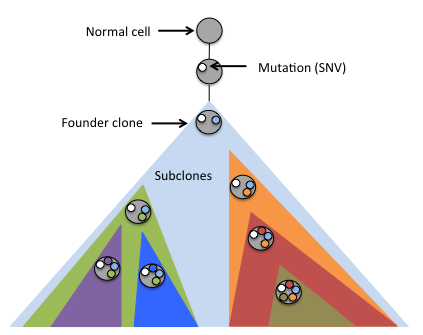
\includegraphics[width=0.65\textwidth]{images/heterogeneity.png}}
\footnotetext[1]{El-Kebir 2015}
\end{frame}

% Slide 2
\begin{frame}{Clinical significance.}
\centerline{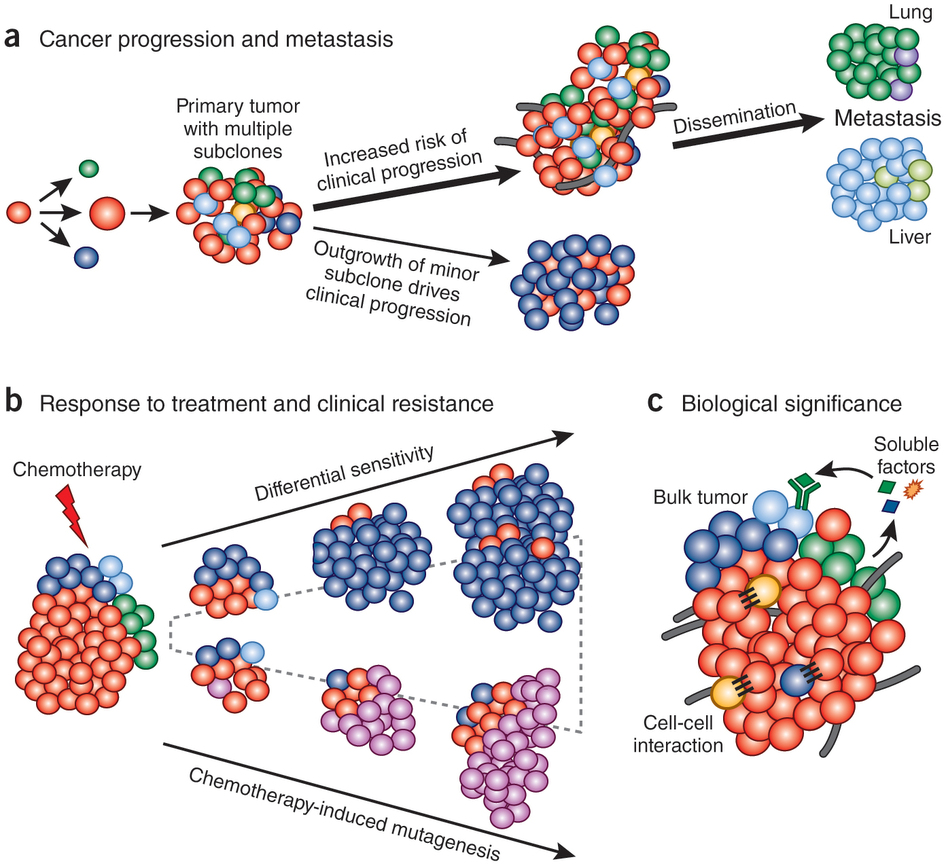
\includegraphics[width=0.75\textwidth]{images/heterogeneity_significance.jpg}}
\footnotetext[1]{Kleppe 2014}
\end{frame}

% Slide 3
\begin{frame}{Clonal mixture from bulk-sequencing data.}
\begin{itemize}
	\item We observe DNA bulk-sequencing data.
		\begin{itemize}
			\item Reference and variant reads.
		\end{itemize}
	\pause
	\vspace{0.15in}
	\item Cluster mutations that occur with similar frequency.
	\begin{itemize}
		\item Mutations from the same cluster should occur with the same frequency.
	\end{itemize}
\end{itemize}
\end{frame}

% Slide 4
\begin{frame}{Multiple samples increase resolution.}
\centerline{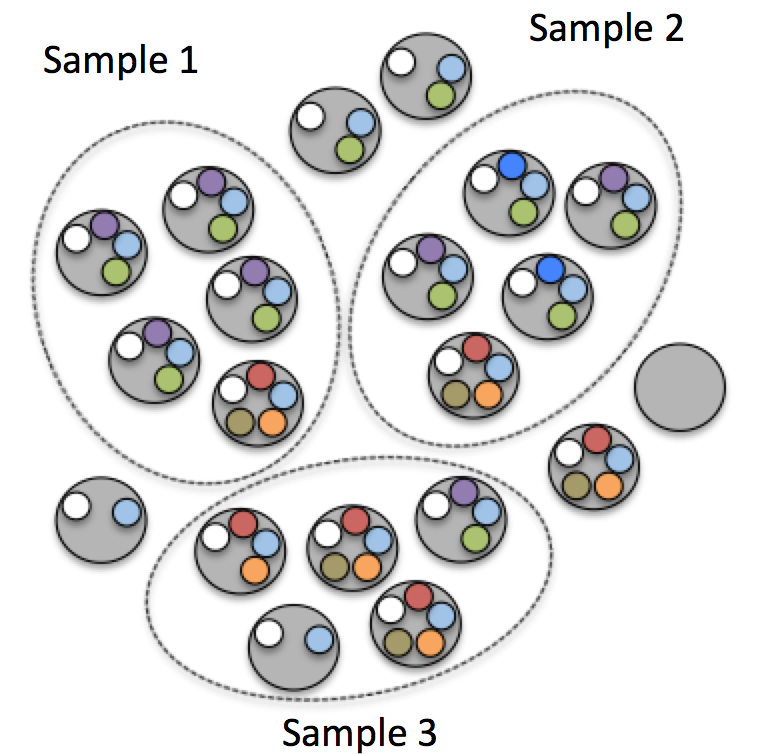
\includegraphics[width=0.55\textwidth]{images/multiplesamples.png}}
\end{frame}

%%%%%%%%%%%%%
% The model
%%%%%%%%%%%%%
\section{Model}
\begin{frame}{Observed data}
Given $n=1,\ldots, N$ SNVs, and $m=1,\ldots,M$ samples, we are given:
%\pause
%\begin{definition}[Variant Allele Frequency]
%The \alert{variant allele frequency (VAF)} for a SNV $n$ in sample $m$ is 
%\end{definition}
\begin{itemize}
	\pause
	\item Variant reads, $v_{mn}$ \pause
	\item Total reads, $d_{mn}$
\end{itemize}
\bigskip
\pause So for each SNV, we can vectorize across samples: \pause
\begin{align*}
\bm{d_{n}} &\triangleq 	\begin{bmatrix} d_{1n} \\ d_{2n} \\ \vdots \\ d_{Mn} \end{bmatrix}, \quad\bm{v_{n}} \triangleq 	\begin{bmatrix} v_{1n} \\ v_{2n} \\ \vdots \\ v_{Mn} \end{bmatrix}.
\end{align*}
\pause
Let $\bx_{n}$ be general notation for $\{\bm{d}_{n}, \bm{v}_{n}\}$, where the use of the total or variant reads will be clear from context.
\end{frame}

\begin{frame}{Assigning mutations to clusters}
Suppose that each SNV $n \in \{1, ..., N\}$ belongs to a cluster $k\in\{1,\ldots,K\}$, $K \leq N$.
\pause
\begin{itemize}
	\item<2-> Latent variables $\bz_n$, a 1-of-$K$ indicator vector that denotes the cluster assignment of SNV $n$ to cluster $k$. 
	\item<3-> We don't know the number of clusters in advance.
\end{itemize}
\end{frame}

\begin{frame}{Problem statement}
\begin{block}{SNV clustering problem}
Suppose that for SNVs $n \in \{1, ..., N\}$ in samples $m\in\{1, \ldots M\}$. Further suppose that there exists clones (clusters) $k\in\{1,\ldots,K\}$ and a true clustering $\bz$. Given total reads $\bm{d}_1, \ldots, \bm{d}_n$ and variant reads $\bm{v}_1, \ldots, \bm{v}_n$, we seek to infer $\bm{z}$.
\end{block}
\end{frame}

\begin{frame}{Observation model}
Now suppose that the variant reads are binomially distributed.
\begin{itemize}
	\item<2-> Each cluster emits variant reads with \emph{cluster frequency} $\phi_{mk}$.
	\item<3-> Then \begin{align*}
	\bf{v}_{n} &\sim
				\begin{bmatrix}
					\mathrm{Bin}(v_{1n}; d_{1n}, \bphi_{1k}) \\ \mathrm{Bin}(v_{2n}; d_{2n}, \bphi_{2k}) \\ \vdots \\ \mathrm{Bin}(v_{Mn}; d_{Mn}, \bphi_{Mk})
				\end{bmatrix}
				\triangleq \bm{\mathrm{Bin}(\bphi_k)}
\end{align*}
\end{itemize}
\end{frame}

\begin{frame}{Dirichlet Process}
\begin{definition}[Dirichlet Process]
For any measurable finite partition $\left\{B_i\right\}_{i=1}^{n}$ of a measurable set $S$ ,
\begin{align*}
&\text{if } X \sim \mathrm{DP}\left(H, \alpha\right) \\
&\text{then }\left(X\left(B_1\right),\dots,X\left(B_n\right)\right) \sim \mathrm{Dir}\left(\alpha H\left(B_1\right),\dots, \alpha H\left(B_n\right)\right)
\end{align*}
where $\mathrm{Dir}$ denotes the Dirichlet distribution.
\end{definition}
\begin{itemize}
	\item<1-> A non-parametric prior on the number of clusters.
\end{itemize}
\end{frame}

\begin{frame}{Dirichlet Process}
It is convenient to represent the Dirichlet Process in terms of its stick-breaking representation:
\begin{align*}
\pi_i(\mathbf{v}) &= v_i \prod\limits_{j=1}^{i-1} (1 - v_j) \\
				DP &= \sum_{i=1}^\infty \pi_i(\mathbf{v}) \delta_{\phi_i}
\end{align*}
where $\phi_i$ are the parameters for the realized distribution, and $v_i$ are iid $\mathrm{Beta}(1, \alpha)$. \\[6pt]
We will use the stick breaking representation here.
\end{frame}

\begin{frame}{Binomial Mixture Model with DP prior}
Likelihood of data given its cluster membership:
\begin{equation*} \label{eq:xlikelihood}
\Pr(\mathbf{x_n} | \bphi_k) = \prod\limits_{m=1}^M \mathrm{Bin}(v_{mn}; d_{mn}, \bphi_k)
\end{equation*}

%Likelihood of data given latent variables:
%\begin{align*} \label{eq:jointlikelihood}
%\Pr(\mathbf{x_n} | \bz, \bphi_k) &= \prod\limits_{k=1}^K \Pr(\mathbf{x_n} | \mathbf{\phi_k})^{\bz_{nk}} \nonumber \\
%										&= \prod\limits_{k=1}^K \prod\limits_{m=1}^M \mathrm{Bin}(v_{mn}; d_{mn}, \bphi_{mk})^{\bz_{nk}}
%\end{align*}
\pause
Joint likelihood of observed data and cluster memberships:
\begin{equation*}
\Pr(\mathbf{x_n}, \bz | \bm{\pi}, \bphi) = \prod\limits_{k=1}^K \prod\limits_{m=1}^M \left(\pi_k \mathrm{Bin}(v_{mn}; d_{mn}, \phi_{mk})\right)^{\bz_{nk}}
\end{equation*}
\end{frame}

\begin{frame}{Binomial Mixture Model with DP prior}
\centerline{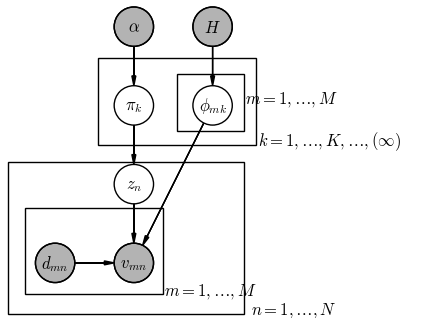
\includegraphics[scale=0.70]{images/multi_pgm.png}}
\end{frame}

\begin{frame}{Binomial Mixture Model with DP prior}
The full cluster assignment posterior 
\begin{equation*}
p(\bz | \bx, \alpha, H) = \int p(\bx | \mathbf{\phi}) p(\phi | \bx, \alpha, H) \, d\phi
\end{equation*}
involves a Dirichlet Process and is thus analytically intractable. We must use some sort of computational technique, such as variational inference, to perform inference on this posterior.
\end{frame}

%%%%%%%%%%%%%
% Variational Inference
%%%%%%%%%%%%%

\section{Inference}

\begin{frame}{Variational Inference}
\emph{Variational Inference} (VI) is an alternative to MCMC sampling-based inference methods.
\vspace{0.05in}
\begin{itemize}
	\item<2-> Generalized version of EM; deterministic given an initialization.
	\item<3-> Faster than MCMC.
	\item<4-> Scales well on large datasets.
\end{itemize}
\end{frame}

\begin{frame}{Overview of Variational Inference: I}
Let $\mathbf{z}$ denote the latent variables, and $\mathbf{x}$ denote the data. We seek to approximate the posterior $p(\mathbf{z}|\mathbf{x})$ from a family of distributions $\mathcal{D}$ by solving the following optimization problem: 
\begin{equation*} \label{eq:optimalq}
q^*(z) = \arg\!\min_{q(\mathbf{z}) \in \mathcal{D}} \kl{(q(\mathbf{z}) || p(\mathbf{z}|\mathbf{x}))}.
\end{equation*}
where \textsc{kl} is the KL-divergence, which measures the ``distance'' between two distributions. \footnotetext[1]{Blei 2006}
\end{frame}

\begin{frame}{Overview of Variational Inference: II}
However, the KL-divergence requires us to compute the log evidence (which is intractable over the space of all $\mathbf{z}$), since
\begin{align*}
  \kl{q(\bz) \| p(\bz \g \bx)} =
  \E\left[\log q(\bz)\right] -
  \E\left[\log p(\bz, \bx)\right] +
  \log p(\bx). 
\end{align*}
\pause
Instead, we optimize the an objective function which is not dependent on $\log p(\bx)$, called the evidence lower bound (\textsc{ELBO}):
\begin{align*}
  \ELBO(q) =
  \E{[\log p(\bz, \bx)]} -
  \E{[\log q(\bz)]}.
\end{align*}
The $\textsc{ELBO}$ is a lower bound for the $\log$ evidence. 
\end{frame}

\begin{frame}{Overview of Variational Inference: III}
The standard technique is to select a simple family of distributions for $\mathcal{D}$, the mean-field variational family. In this family, the latent variables $\bz$ are mutually independent so that the joint distribution factorizes:
\begin{align*}
  q(\bz) = \prod_{j=1}^{m} q_j(z_j).
\end{align*}
where $q_j$ is a bounded variation dependent only on $z_j$. The structure of the model will dictate the optimal form of $q_j$. 
\end{frame}

\begin{frame}{Overview of Variational Inference: IV}
The mean-field assumption gave us independence between variables. This suggests a coordinate ascent algorithm. \pause

\medskip
Let $\bz_{-j}$ denote the set of latent variables $\bz_l$ such that $l \neq j$. Then we can show that
	 \begin{align*}
\ELBO(q) &= \int \prod q_i(\bz_i) \left(\log p(\bz, \bx) - \sum_i \log q_i(\bz_i) \right) \,d\bz \nonumber \\
			&\propto \int q_j(z_j) \E_{-j}\left[\log p(\bx, \bz) \right] \, d\bz_j - \int q_j(z_j) \log q_j(\bz_j) \, d\bz_j
\end{align*}
\pause
Now suppose that we fix $z_{-j}$ and maximize the \textsc{ELBO}. It can be shown that 
\begin{align*}
q^*_j(\bz_j) \propto \exp\left(\E_{-j}\left[\log p(\bx, \bz) \right]\right)
\end{align*}
\pause
By iterating through these coordinate updates, we reach a local optimum of the \textsc{ELBO}.
\medskip
 \footnotetext[1]{Bishop 2006}
\end{frame}

\begin{frame}{Overview of Variational Inference: V}
If the posterior is in the exponential family, then the computation of coordinate ascent and ELBO can be generalized. \\[10pt]
\pause
Recall that a distribution is in exponential form if it can parameterized by 
\begin{equation*}
f_X(x\mid\theta) = h(x) \exp \left (\theta^T \cdot T(x) -A(\theta)\right )
\end{equation*}
where $T(x)$ are the sufficient statistics, $\theta$ are the natural parameters,$A(\theta)$ is the cumulant, and $h(x)$ is the base measure. 
\\[10pt]
\pause
The intuition is that because $q^* \propto \exp(\E[\log(.)])$, then writing the distribution in exponential form reveals dependencies that hold for all exponential family members.
 \footnotetext[1]{Hughes 2015}
\end{frame}

\begin{frame}{Overview of Variational Inference: VI}
So why not always use variational inference? \vspace{0.1in}
\begin{itemize}
\setlength\itemsep{1em}
	\item<2-> Accuracy depends on quality of approximation.
		\begin{itemize}
			\setlength\itemsep{0.25em}
			\setlength\topsep{0.5em}
			\item<3-> $q^*$ might be far off from the true posterior.
			\item<4-> MCMC is potentially more accurate...but it might get stuck in local optima or take forever to converge.
		\end{itemize}
	\item<5-> MCMC, like Gibbs sampling, is typically easier to implement.
		\begin{itemize}
			\item<6-> No need for painful derivations.
		\end{itemize}		
\end{itemize}
\end{frame}

%%%%%%%%%%%%%
% Methods
%%%%%%%%%%%%%
\section{Methods}
\begin{frame}{Existing methods}
\centerline{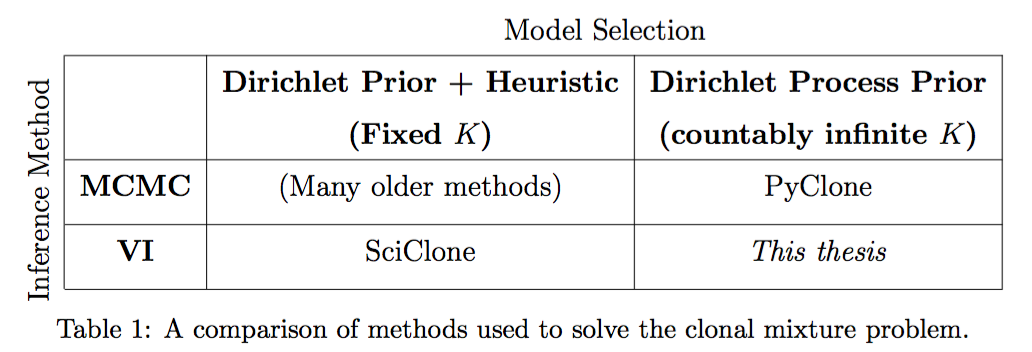
\includegraphics[scale=0.55]{images/methodstable.png}}
\end{frame}

\begin{frame}{VI for the DP/Binomial mixture model}
By beta-binomial conjugacy, 
\begin{align*}
q(\bm{\phi}_k)  &= \prod\limits_{m=1}^M q(\bm{\phi}_{mk}) \\
				&= \prod\limits_{m=1}^M \mathrm{Beta}(\bm{\phi}_k | \alpha_{mk}, \beta_{mk})
\end{align*}
\pause
Thus, combined with the DP variational parameters,
	\begin{gather}
	\begin{align}
	    q(\bz, \mathbf{v}, \bm{\phi}) &=
	\underbrace{\prod\limits_{k=1}^K q(\bm{\phi}_k)}_{\substack{\text{Observation: likelihoods}  \\  \text{Product of betas} \\ 2MK \text{ variational parameters} \\  \{\alpha_{mk}, \beta_{mk} \}_{m=1, k=1}^{M, K} }} \times
	 \underbrace{\prod\limits_{k=1}^K q(\mathbf{v}_k)}_{\substack{\text{Allocation: cluster proportions} \\ \text{Product of betas} \\ 2K \text{ variational parameters}  \\ \{\eta_{k0}, \eta_{k1}\}_{k=1}^K   }} \times
	 \underbrace{\prod\limits_{n=1}^{N} q(z_n)}_{\substack{ \text{Allocation: cluster responsibilities} \\ \text{Product of categoricals} \\ 2NK \text{ variational parameters}  \\ \{\hat{r}_{nk}\}_{n=1, k=1}^{N, K}   }}\nonumber
	 \end{align}
	\end{gather}
Most of the details are in the thesis appendices.
\end{frame}

\begin{frame}{MAP estimates}
For each cluster we pool reads by cluster membership:
\begin{align*}
v_{mk}^{\text{pooled}} &= \sum_n (v_{mn})^{\bz_n} \\
d_{mk}^{\text{pooled}} &= \sum_n (d_{mn})^{\bz_n}
\end{align*}
\pause
and we can make MAP estimates by converting from the variational parameters back to the original parameters of the posterior:
\begin{align*}
\bz_n^{\text{MAP}} &= \arg \max_k \hat{r}_{nk}  \\[8pt]
\phi_{mk}^{\text{MAP}} &= \frac{v_{mk}^{\text{pooled}} + \alpha_{mk} - 1}{d_{mk}^{\text{pooled}} + \alpha_{mk} + \beta_{mk} - 2}.
\end{align*}
\end{frame}

\begin{frame}{Implementation}
\pause
\begin{itemize}
	\item Responsibilities initialized with k-means$++$ on $N$ clusters.
	\item\pause Uniform priors for the betas.
	\item\pause DP hyperparameters chosen empirically.
\end{itemize}
\pause We declared convergence when the difference in ELBO between two iterations was less than 0.01. \\[6pt]
\pause
Everything was implemented in Python.
\end{frame}

\begin{frame}{Coordinate ascent algorithm}
\vspace{-0.15in}
  \begin{center}
    \scalebox{0.65}{
    \begin{minipage}{1.25\linewidth}
\begin{algorithm}[H]
\SetCommentSty{itshape}
\KwIn{Data $\bx_n$, where each $x_i$ is an integer vector with $M$ entries. \\ \hspace{1.25cm} $\gamma_0, \gamma_1, \alpha_0, \beta_0$, hyperparameters}
\vspace{0.1cm}
\KwOut{Converged variational parameters $\{\alpha_{mk}, \beta_{mk} \}_{m=1, k=1}^{M, K}, \{\eta_{k0}, \eta_{k1}\}_{k=1}^K, \{\hat{r}_{nk}\}_{n=1, k=1}^{N, K}$}
	\vspace{0.1cm}
\textbf{Initialize:}     $\alpha_0 = \beta_0 = \alpha_{mk} = \beta_{mk} = 1$, $\forall m, k$ \\
\hspace{1.85cm}    $\gamma_1 = \eta_1 = 1.0, \gamma_0 = \eta_0 =1.5$ \\
\hspace{1.85cm}    $\hat{r}_{nk} \leftarrow \texttt{kmeans++}(\bx)$ \\
	\vspace{0.1cm}
\While{the \textsc{ELBO} has not converged} {
	\vspace{0.05cm}
	\Comment*[h]{Compute data-specific (local) parameters} \\
		\hspace{1cm} $\E_q[\log p(x_n | \alpha_{mk}, \beta_{mk})] \leftarrow \E_q[\log \left( \binom{d_{mn} + v_{mn}}{v_{mn}} (\bm{\phi}_k)^{v_{mn}} (1-\bm{\phi}_k)^{d_{mn}} \right)]$ \\
		\hspace{1cm} $\hat{r}_{nk} \leftarrow \exp(S_k)$ \\
		
	\vspace{0.1cm}	
	\Comment*[h]{Compute sufficient statistics} \\
		 \hspace{1cm} $S_k = \sum_{n=1}^N \hat{r}_{nk} s(x_n) = \sum_{n=1}^N \hat{r}_{nk} \begin{bmatrix}
				\begin{bmatrix}
				 v_{1n} &  d_{1n}
				\end{bmatrix} & \cdots &
				\begin{bmatrix}
				 v_{Mn} &  d_{Mn}
				\end{bmatrix}
			\end{bmatrix}$ \\
		\hspace{1cm} $N_k = \sum_{n=1}^N \hat{r}_{nk}$ \\
		\hspace{1cm} $N_k^> = \sum_{k+1}^K N_k$
	
	\vspace{0.1cm}	
	\Comment*[h]{Compute cluster-specific (global) parameters} \\
		\hspace{1cm} $\eta_{k1} \leftarrow 1 + \sum_n \hat{r}_{nk} = 1 + N_k$ \\
		\hspace{1cm} $\eta_{k0} \leftarrow \gamma + \sum_n \sum_{j=k+1}^K \hat{r}_{nj} = N_k^>$\\
%		\hspace{1cm} $[\bm{\alpha}_{k}, \bm{\beta}_{k}] \leftarrow [(\alpha_0 - 1), (\beta_0 - 1)] + S_k $ \\
		\hspace{1cm} $\alpha_{mk} \leftarrow  (\alpha_0 - 1) + S_{km}$ \\
		\hspace{1cm} $ \beta_{mk} \leftarrow (\beta_0 - 1) + S_{km}$ \\
	\vspace{0.1cm}		
  Compute $\ELBO(q) = \EE{\log p(\bz, \bx)} - \EE{\log q(\bz)}$
}
\Return{Converged variational parameters}
\caption{\textsc{CAVI for the DP Binomial mixture model}}
\label{alg:cavi}
\end{algorithm}
    \end{minipage}%
    }
  \end{center}
\end{frame}


%%%%%%%%%%%%%
% Results
%%%%%%%%%%%%%
\section{Results}
\begin{frame}{Simulated Data}
\begin{table}[ht]
\centering
\begin{tabular}{| l | l |}
\hline
Number of clusters ($K$) & 10            \\ \hline
Number of SNVs ($N$)     & 100           \\ \hline
Number of samples ($M$)  & 4, 5, 6       \\ \hline
Coverage                 & 50, 100, 1000  \\ \hline
\end{tabular}
\end{table}
\centerline{Parameters for the simulated datasets.}
\end{frame}

\begin{frame}{Evaluating results}
The DP/VI coordinate ascent algorithm was benchmarked against SciClone (VI) and PyClone (DP/MCMC). \vspace{0.15in}
\begin{itemize}
	\item Evaluate clustering: Adjusted Rand Index (ARI)
	\item Evaluate parameters: Cluster frequency error (CFE)
		\begin{align*}
		\text{CFE}(\bphi^{\text{MAP}}) \triangleq  \frac{1}{C} \sum_{c=1}^C \min_{k \in \{1, \ldots, K\}}  \left\Vert \bphi_c^{\text{MAP}} - \bphi_k \right\Vert
		\end{align*}
\end{itemize}
\end{frame}

\begin{frame}
	\vspace{-0.075in}
  \begin{center}
    \scalebox{0.85}{
    \begin{minipage}{0.75\linewidth}
\centerline{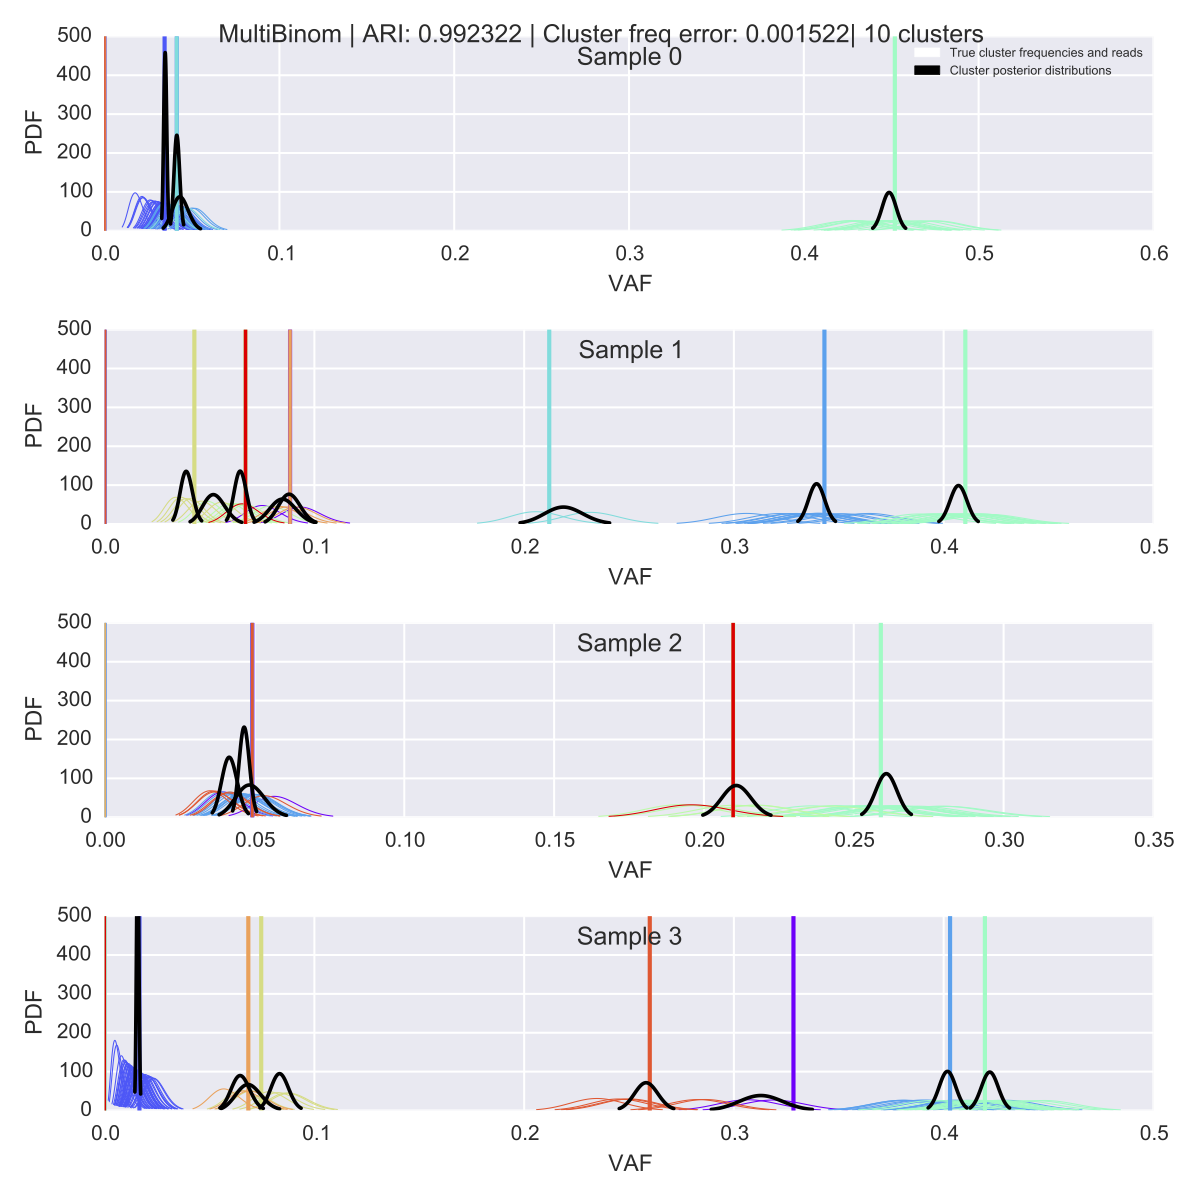
\includegraphics[scale=0.5]{images/example_indiv_plot.png}}
    \end{minipage}%
    }
  \end{center}
  \vspace{-0.20in}
  \hspace{0.3in} \emph{\tiny{Cluster posteriors (black) and true clusters (colored, vertical lines) with $\bx_n$ (colored beta curves).}}
\end{frame}

\begin{frame}{Cluster Frequency Error}
\vspace{-0.05in}
\centerline{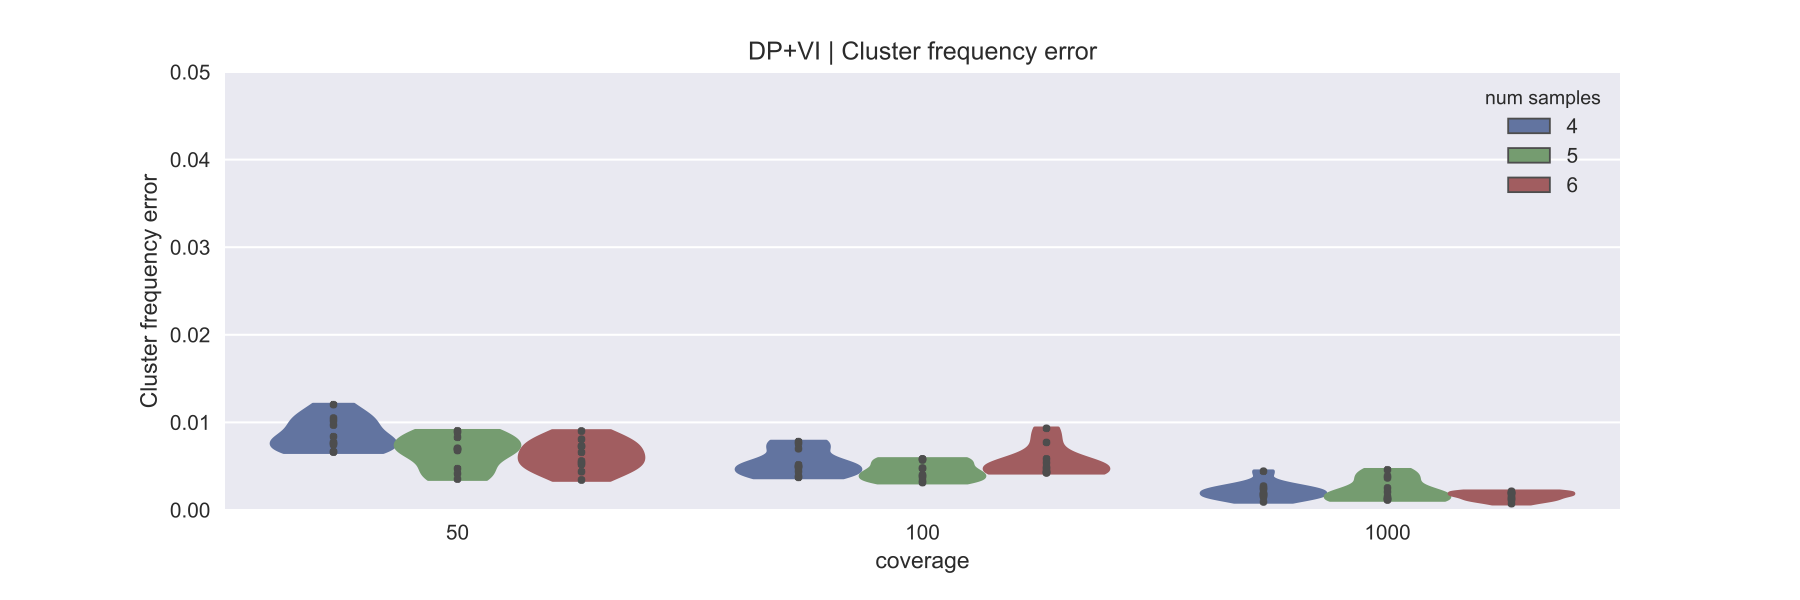
\includegraphics[scale=0.27]{images/DPVI_CFE.png}}
\vspace{-0.05in}
\centerline{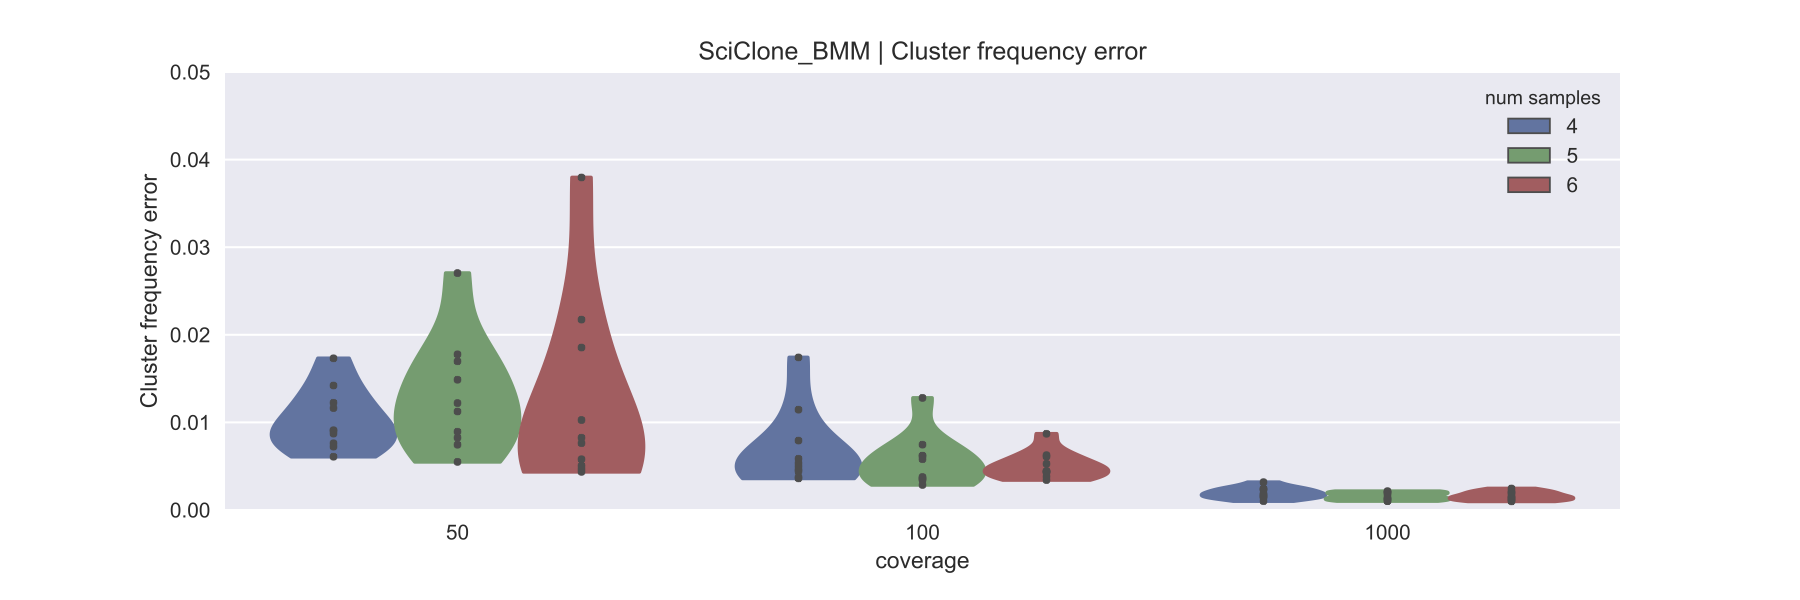
\includegraphics[scale=0.27]{images/SciClone_CFE.png}}
\vspace{-0.05in}
\centerline{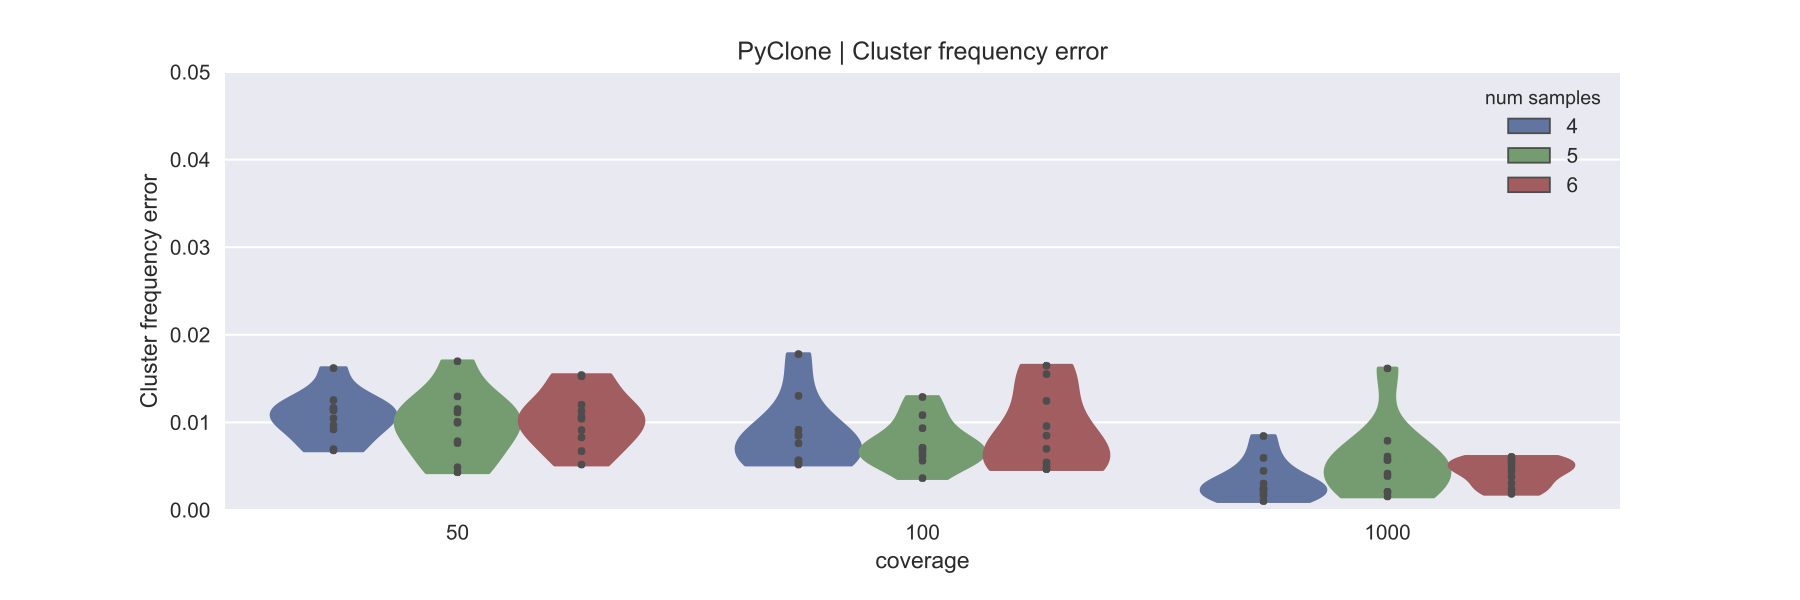
\includegraphics[scale=0.27]{images/PyClone_CFE.png}}
\end{frame}

\begin{frame}{Adjusted Rand Index}
\vspace{-0.05in}
\centerline{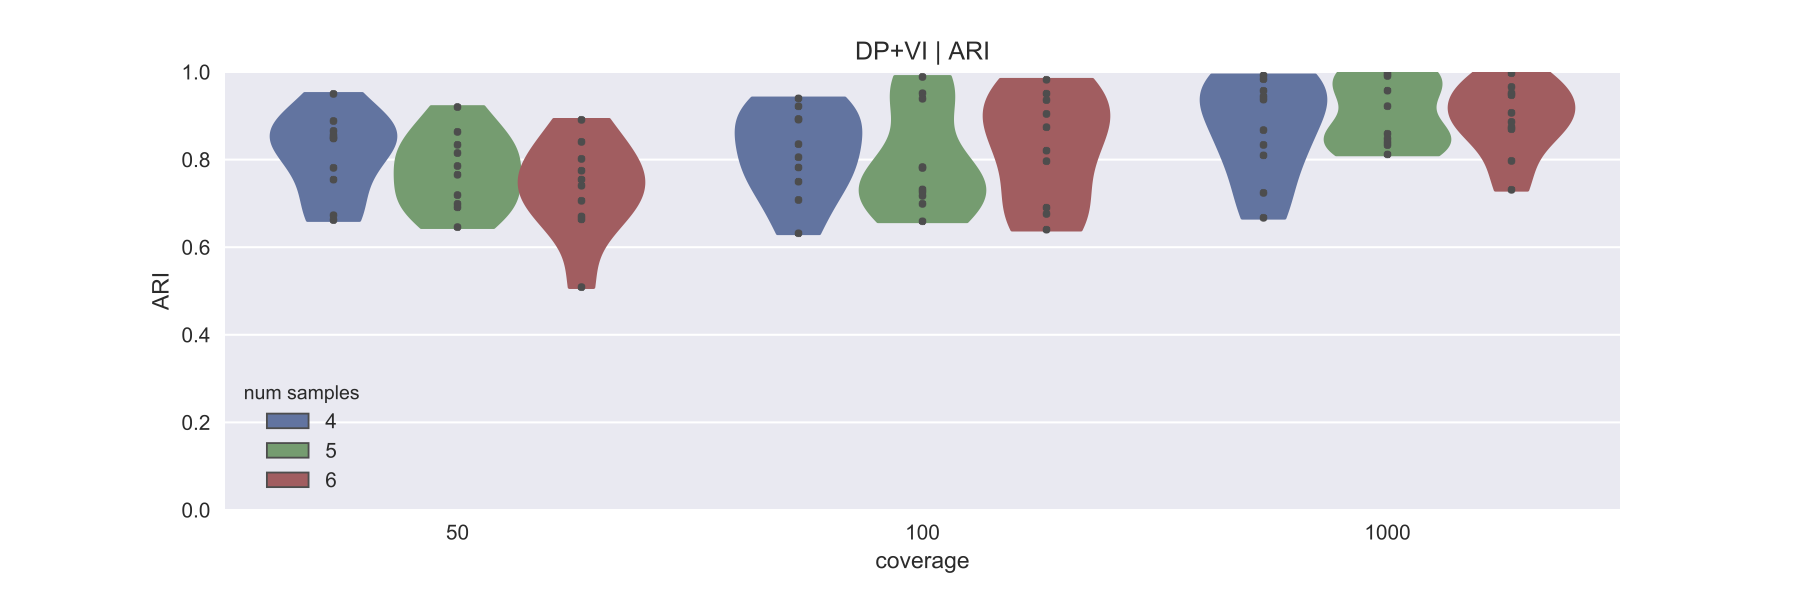
\includegraphics[scale=0.27]{images/DPVI_ARI.png}}
\vspace{-0.05in}
\centerline{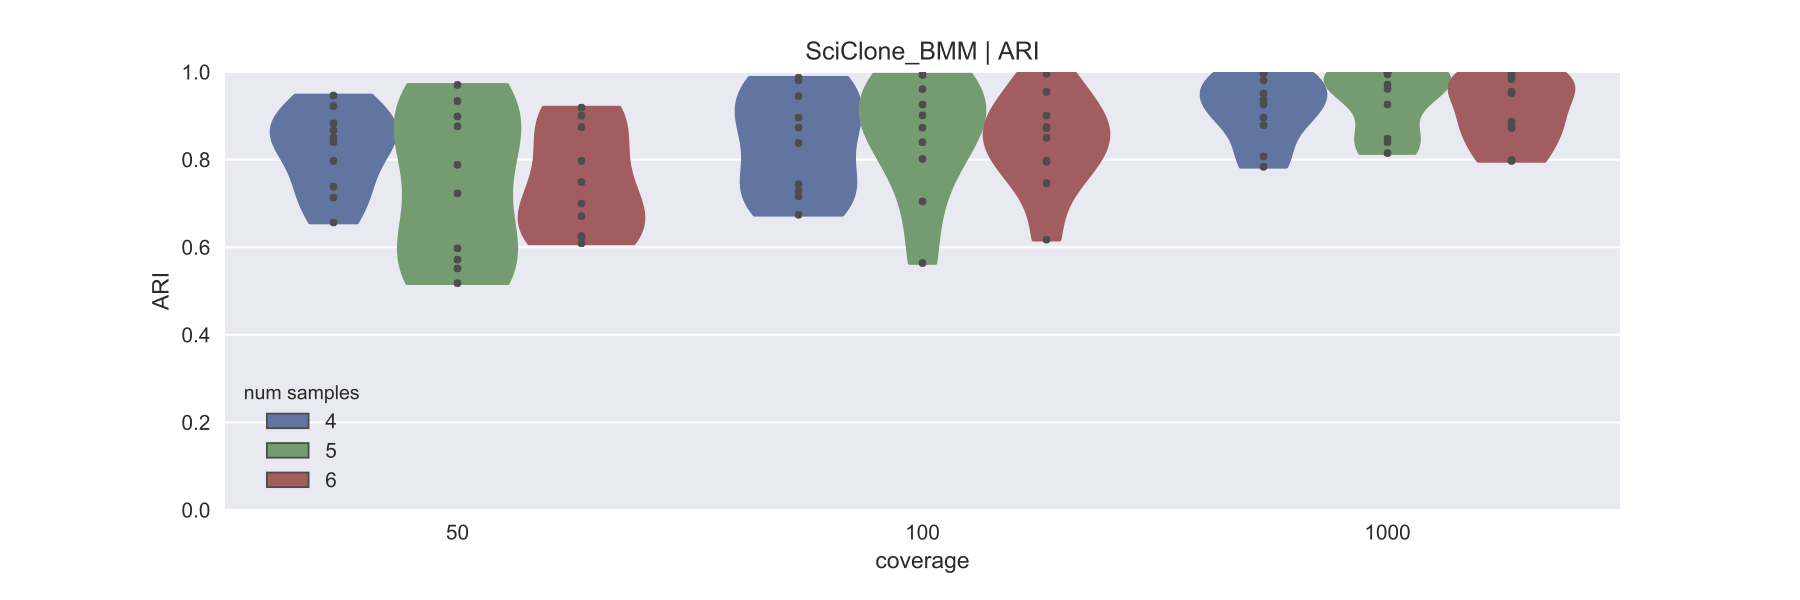
\includegraphics[scale=0.27]{images/SciClone_ARI.png}}
\vspace{-0.05in}
\centerline{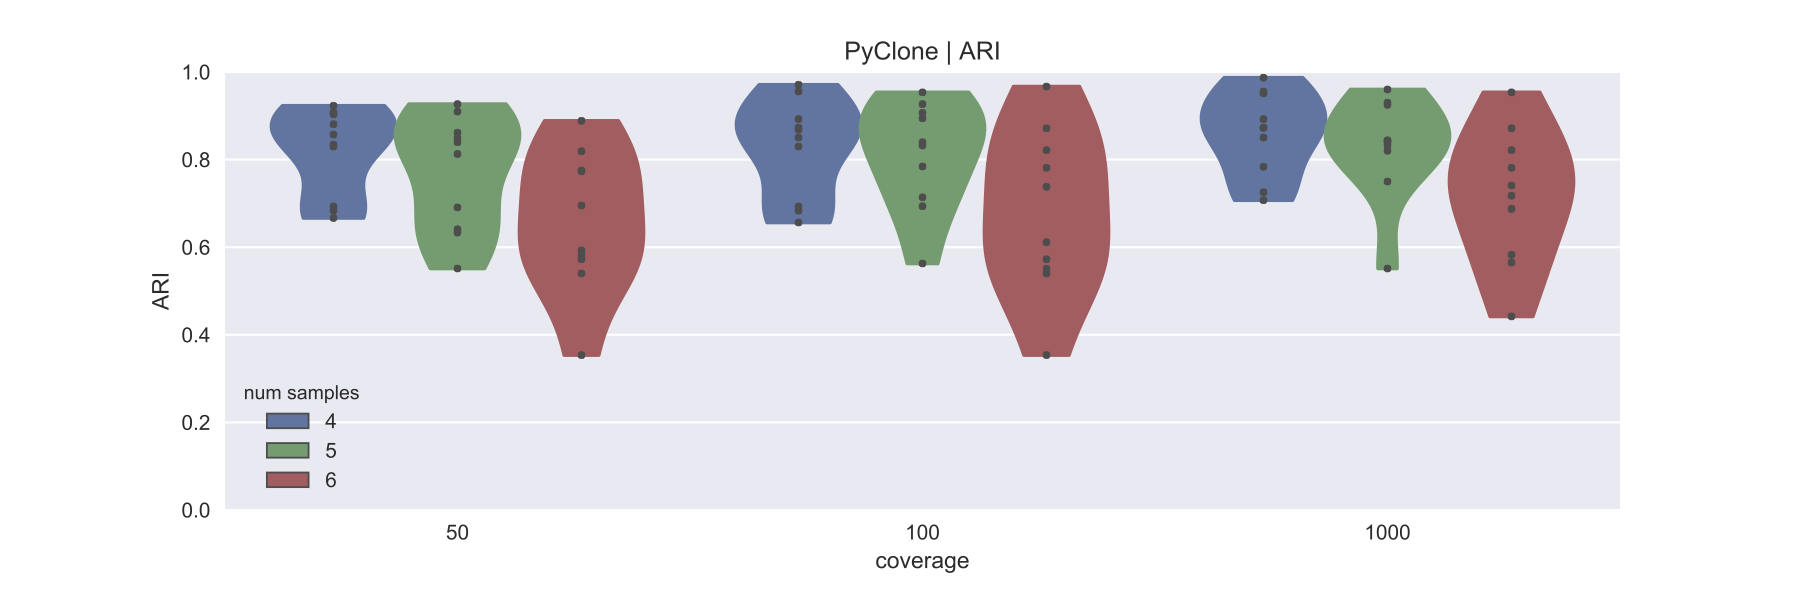
\includegraphics[scale=0.27]{images/PyClone_ARI.png}}
\end{frame}

\begin{frame}{Number of clusters}
\vspace{-0.05in}
\centerline{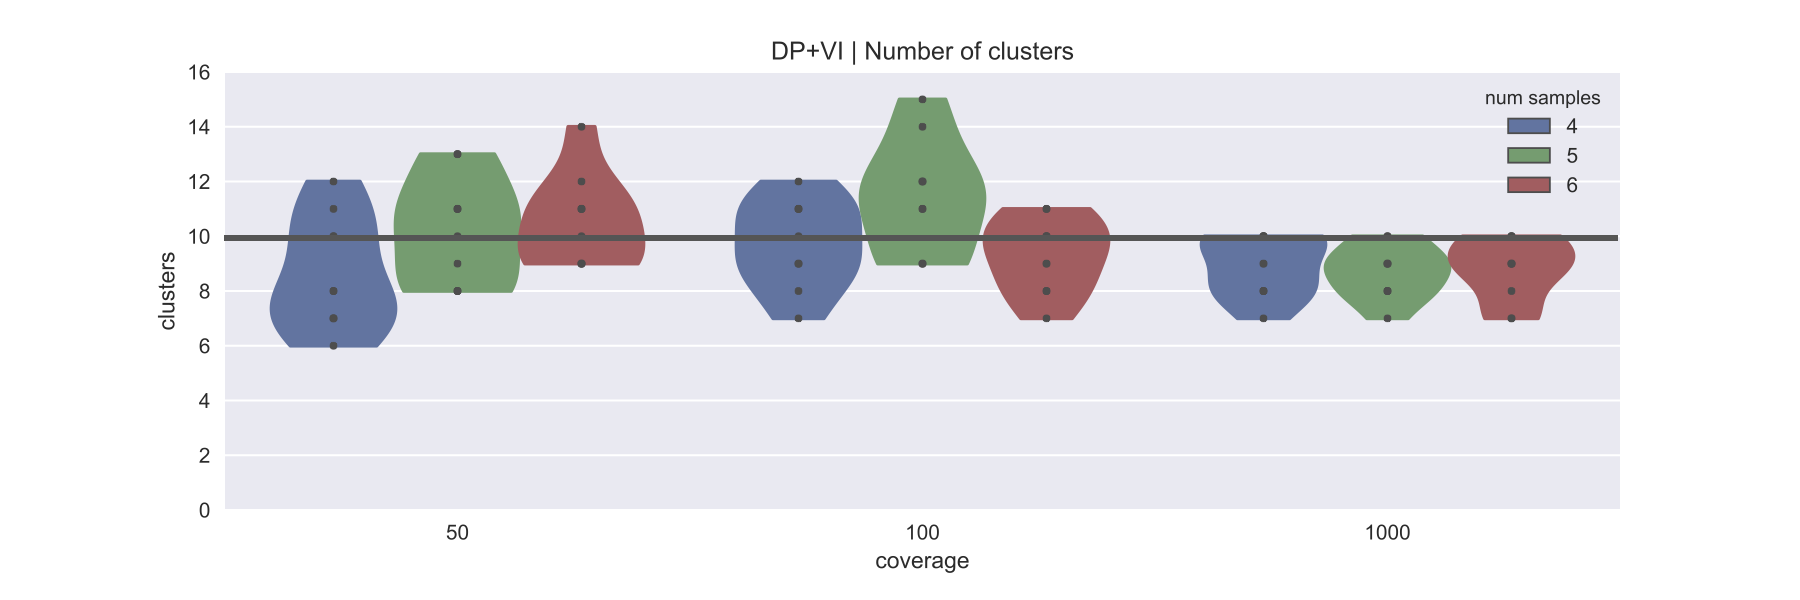
\includegraphics[scale=0.27]{images/DPVI_num_clusters.png}}
\vspace{-0.05in}
\centerline{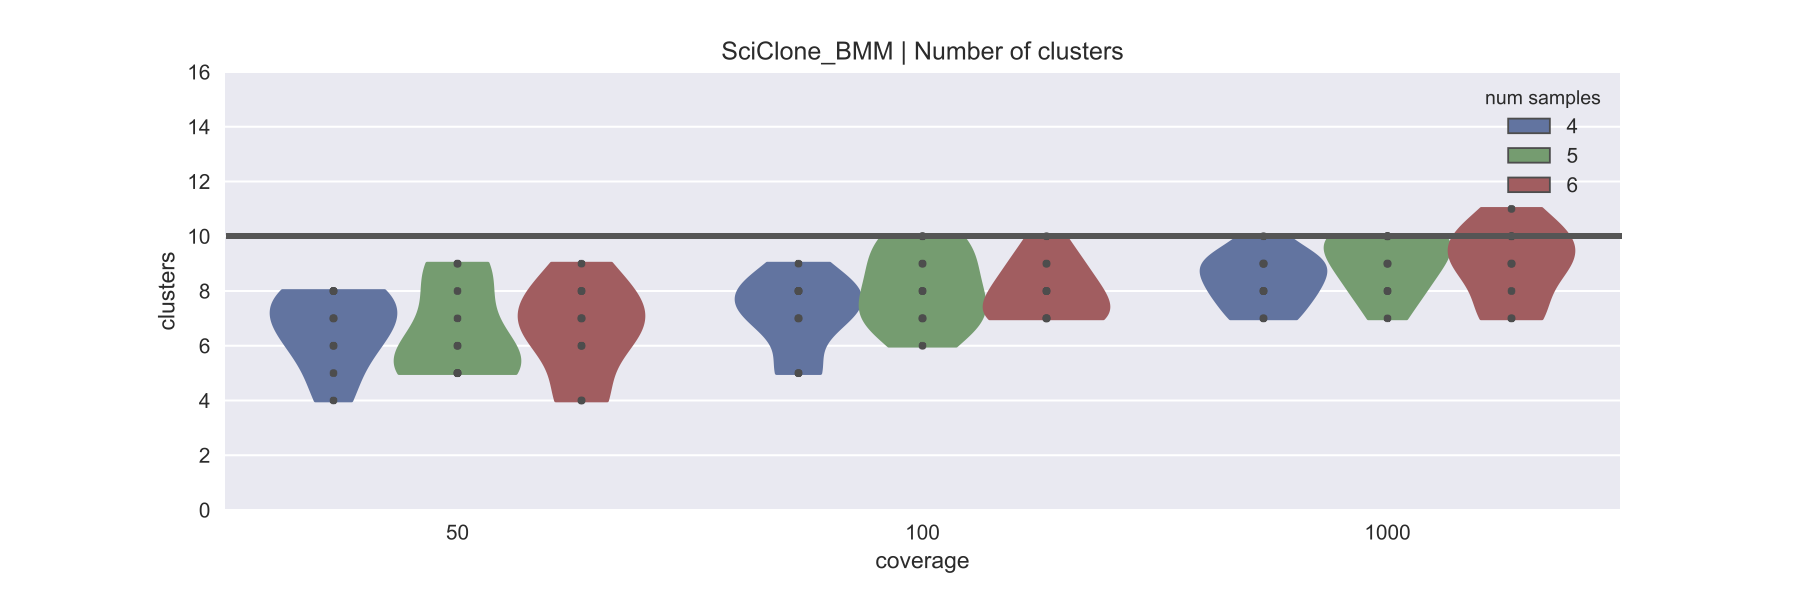
\includegraphics[scale=0.27]{images/SciClone_num_clusters.png}}
\vspace{-0.05in}
\centerline{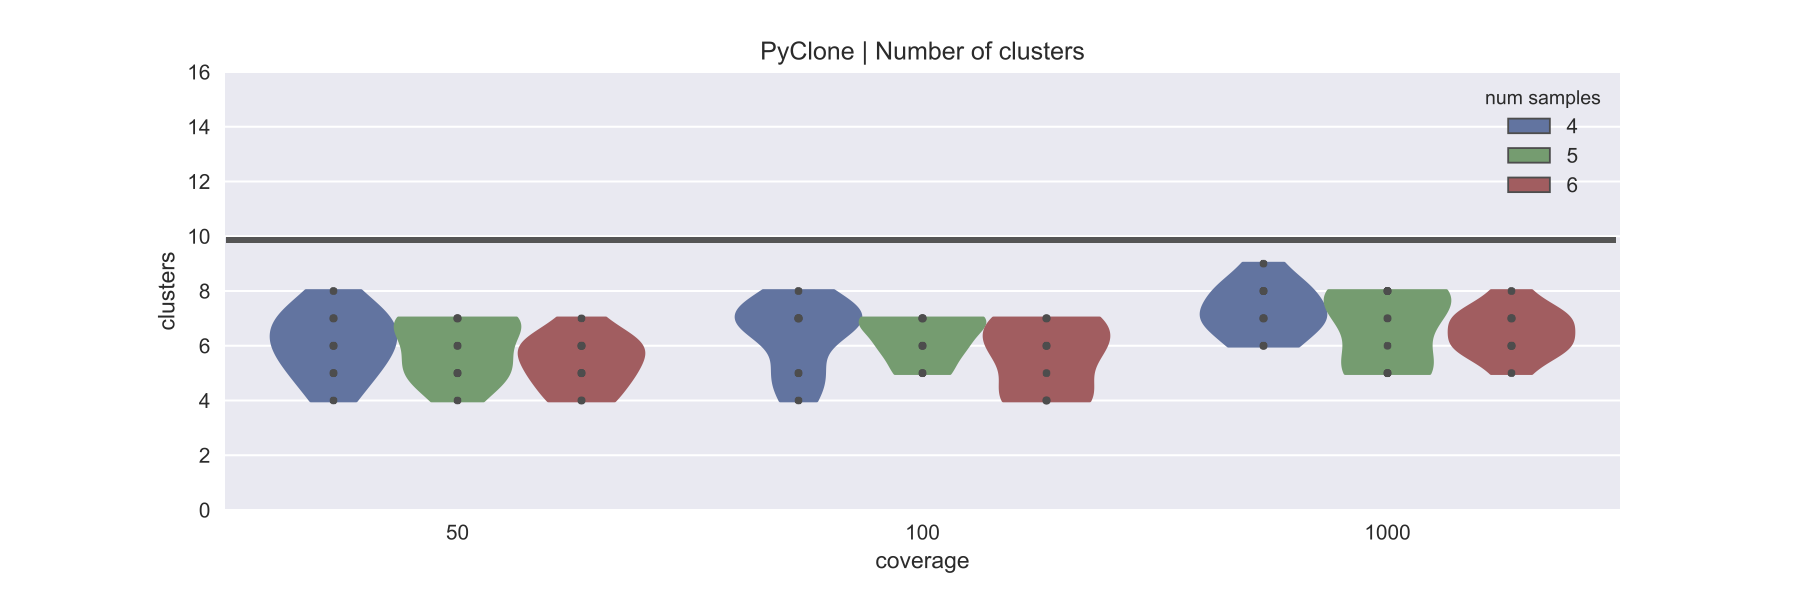
\includegraphics[scale=0.27]{images/PyClone_num_clusters.png}}
\end{frame}

\begin{frame}{Runtime}
\centerline{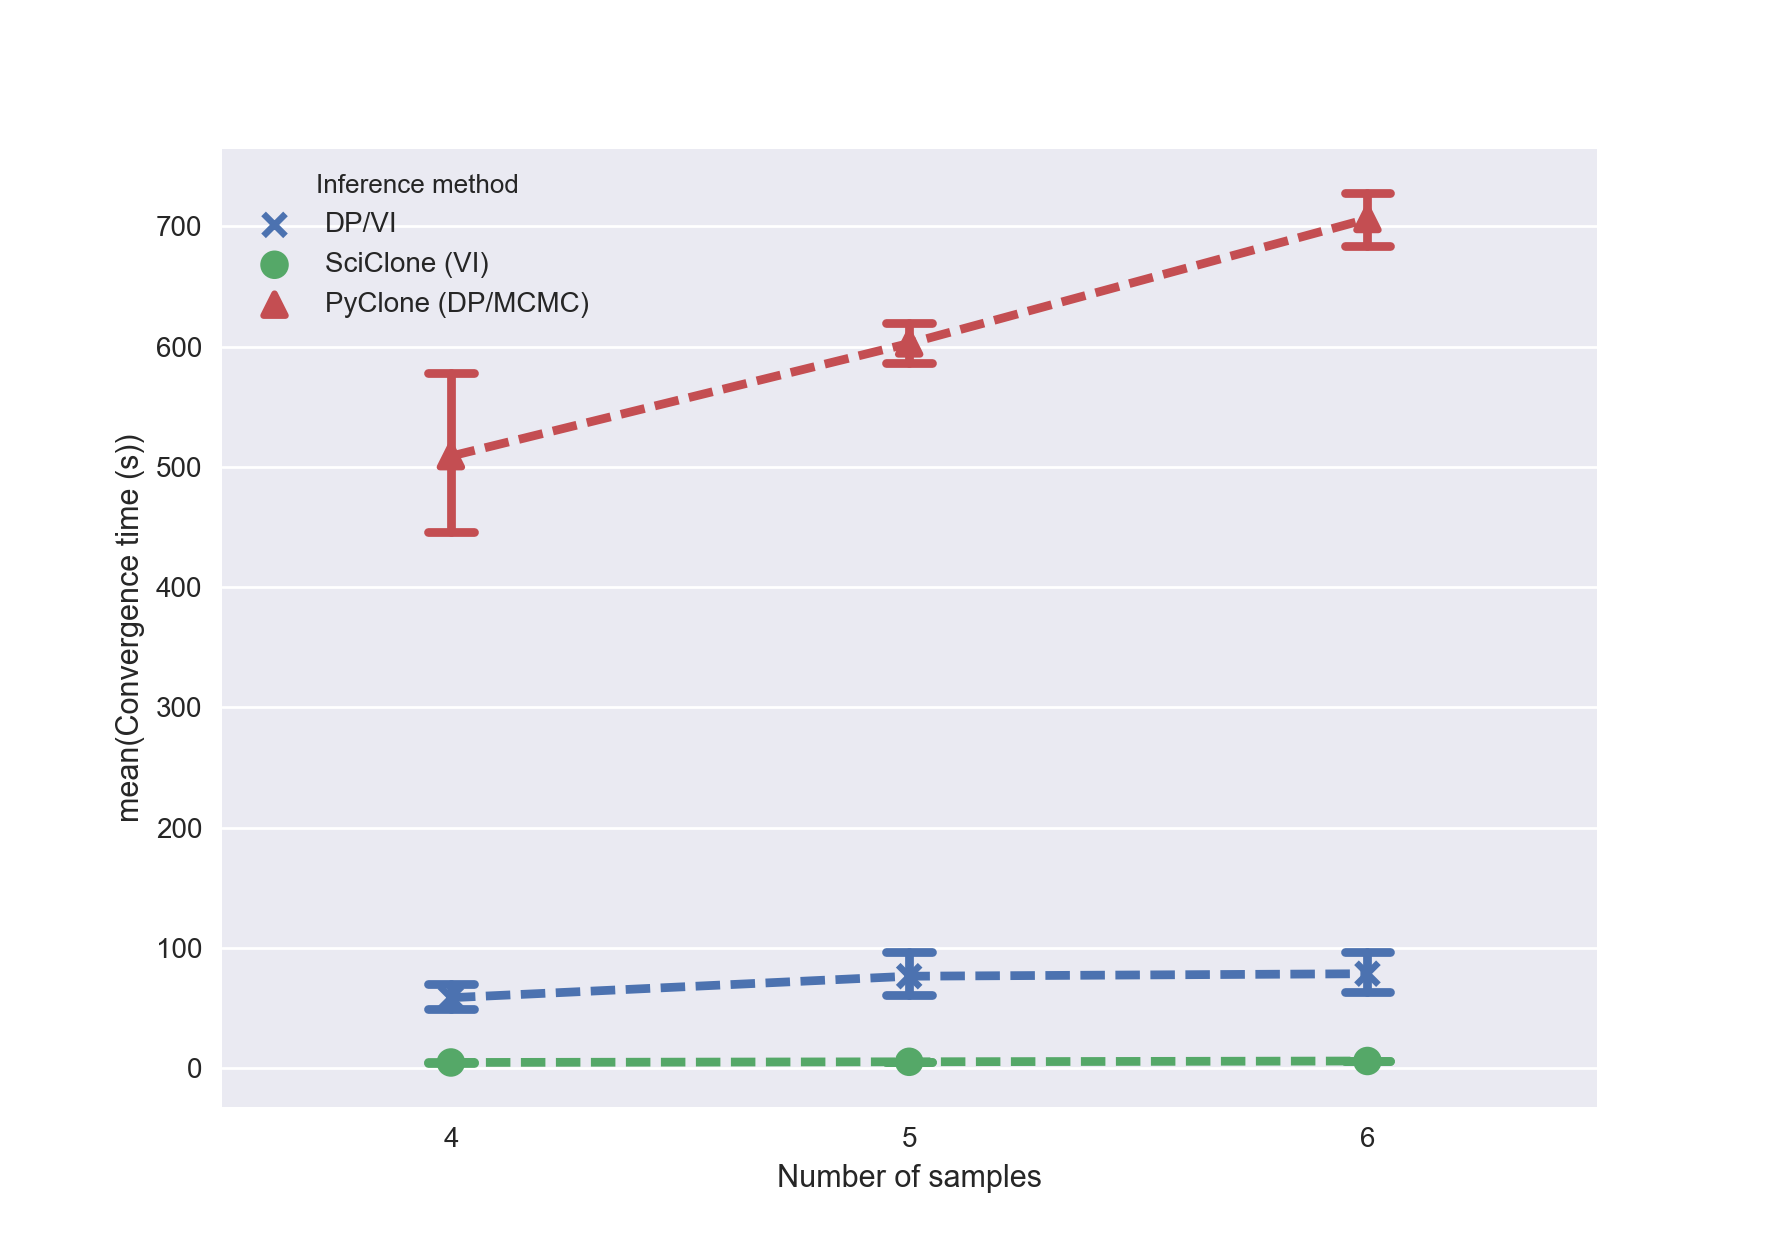
\includegraphics[scale=0.5]{images/time_comparisons.png}}
\end{frame}

%%%%%%%%%%%%%
% Conclusion
%%%%%%%%%%%%%
\section{Conclusion}

\begin{frame}{Discussion}
The DP/VI method is: \vspace{0.1in}
\begin{itemize}
	\setlength\itemsep{1em}
	\item<2-> Faster and more accurate than PyClone (MCMC method)
	\item<3-> Comparable to SciClone (other variational method)
	\begin{itemize}
		\item<4-> Better at lower coverages.
		\item<5-> Added benefit: nonparametric prior.
	\end{itemize}
\end{itemize}
\end{frame}

\begin{frame}{Future Work}
\begin{itemize}
	\setlength\itemsep{0.75em}
	\item<2-> Other models, such as negative binomial
	\item<3-> More advanced variational inference techniques
	\item<4-> Optimize code, write in a faster language
	\item<5-> Try as part of a phylogeny inference pipeline
	\item<6-> Try on real data
\end{itemize}
\end{frame}

\begin{frame}{Acknowledgments}
Thanks to:
\begin{itemize}
	\setlength\itemsep{0.5em}
	\item Prof Ben Raphael
	\item Mohammed El-Kebir, Gryte Satas, and the rest of the Raphael Lab
	\item Prof Erik Sudderth and Mike Hughes
	\item My friends and family
		\begin{itemize}
			\item Especially the support of the others doing theses: \\Uthsav Chitra, Vaki Nikitopoulos, Matt Chin, and Keshav Vemuri
		\end{itemize}
\end{itemize}
\end{frame}

\end{document}